% This template has been adapted from https://github.com/jgm/pandoc-templates
% that comes attached with the following copyright notice. It also includes
% segments from the R Markdown template that in turn is based on the pandoc
% template.
%
% Copyright (c) 2014--2017, John MacFarlane
%
% All rights reserved.
%
% Redistribution and use in source and binary forms, with or without
% modification, are permitted provided that the following conditions are met:
%
% * Redistributions of source code must retain the above copyright notice,
%   this list of conditions and the following disclaimer.
% * Redistributions in binary form must reproduce the above copyright notice,
%   this list of conditions and the following disclaimer in the documentation
%   and/or other materials provided with the distribution.
% * Neither the name of John MacFarlane nor the names of other contributors may
%   be used to endorse or promote products derived from this software without
%   specific prior written permission.
%
% THIS SOFTWARE IS PROVIDED BY THE COPYRIGHT HOLDERS AND CONTRIBUTORS "AS IS"
% AND ANY EXPRESS OR IMPLIED WARRANTIES, INCLUDING, BUT NOT LIMITED TO, THE
% IMPLIED WARRANTIES OF MERCHANTABILITY AND FITNESS FOR A PARTICULAR PURPOSE
% ARE DISCLAIMED. IN NO EVENT SHALL THE COPYRIGHT OWNER OR CONTRIBUTORS BE
% LIABLE FOR ANY DIRECT, INDIRECT, INCIDENTAL, SPECIAL, EXEMPLARY, OR
% CONSEQUENTIAL DAMAGES (INCLUDING, BUT NOT LIMITED TO, PROCUREMENT OF
% SUBSTITUTE GOODS OR SERVICES; LOSS OF USE, DATA, OR PROFITS; OR BUSINESS
% INTERRUPTION) HOWEVER CAUSED AND ON ANY THEORY OF LIABILITY, WHETHER IN
% CONTRACT, STRICT LIABILITY, OR TORT (INCLUDING NEGLIGENCE OR OTHERWISE)
% ARISING IN ANY WAY OUT OF THE USE OF THIS SOFTWARE, EVEN IF ADVISED OF THE
% POSSIBILITY OF SUCH DAMAGE.

\PassOptionsToPackage{unicode=true}{hyperref} % options for packages loaded elsewhere
\PassOptionsToPackage{hyphens}{url}
\PassOptionsToPackage{dvipsnames,svgnames*,x11names*}{xcolor}
%
\PassOptionsToPackage{font=small,
                      labelfont=bf,
                      labelsep=period,
                      justification=RaggedRight,
                      format=plain,
                      tableposition=top,
                      singlelinecheck=off}{caption}

\documentclass[%
numbers=noendperiod,
parskip=half,
bibliography=totoc,
DIV=calc,headsepline=true,
]{scrartcl}

\usepackage{multicol}

% Margin paragraph
\usepackage{marginfix}
%\usepackage{morefloats} % More than 18 floats

\usepackage[font=footnotesize]{subcaption}
\usepackage{booktabs}
\usepackage[document]{ragged2e}
\usepackage[shortlabels]{enumitem}
\usepackage{etoolbox}
\usepackage{floatrow}
\usepackage{environ}
\usepackage{xspace}

\usepackage{ifxetex,ifluatex}


\ifnum 0\ifxetex 1\fi\ifluatex 1\fi=0 % if pdftex

% Fonts

\usepackage[T1]{fontenc}
\usepackage[utf8]{inputenc}
\usepackage{amsthm}
\usepackage[lining]{libertine}
\usepackage{textcomp}
\usepackage[scaled=0.96,varqu,varl]{inconsolata}
\usepackage{mathtools}
\usepackage[libertine,libaltvw,liby,vvarbb]{newtxmath}
\IfFileExists{mathalfa.sty}{\usepackage[scr=boondoxo]{mathalfa}}{}
\IfFileExists{bm.sty}{\usepackage{bm}}{}
\useosf

\else % if luatex or xelatex
  \usepackage{unicode-math}
  \defaultfontfeatures{Ligatures=TeX,Scale=MatchLowercase}
\fi

% use upquote if available, for straight quotes in verbatim environments
\IfFileExists{upquote.sty}{\usepackage{upquote}}{}
% use microtype if available
\IfFileExists{microtype.sty}{%
\usepackage[]{microtype}
\UseMicrotypeSet[protrusion]{basicmath} % disable protrusion for tt fonts
}{}
\IfFileExists{parskip.sty}{%
\usepackage{parskip}
}{% else
\setlength{\parindent}{0pt}
\setlength{\parskip}{6pt plus 2pt minus 1pt}
}
\usepackage{xcolor}
\usepackage{hyperref}
\usepackage{cleveref}
\hypersetup{
            pdftitle={Confidential Neuropsychological Report},
            colorlinks=true,
            linkcolor=PineGreen,
            filecolor=PineGreen,
            citecolor=Periwinkle,
            urlcolor=NavyBlue,
            breaklinks=true}
\urlstyle{same}  % don't use monospace font for urls

% Set tufte-like page layout
\usepackage[
        a4paper,
  left=23mm,
  top=27.4mm,
  bottom=27.4mm,
  textwidth=107mm,
  marginparsep=8mm,
  marginparwidth=49mm]{geometry}

\usepackage{longtable,booktabs}
% Fix footnotes in tables (requires footnote package)
\IfFileExists{footnote.sty}{\usepackage{footnote}\makesavenoteenv{longtable}}{}

\usepackage{graphicx,grffile}
\makeatletter
\def\maxwidth{\ifdim\Gin@nat@width>\linewidth\linewidth\else\Gin@nat@width\fi}
\def\maxheight{\ifdim\Gin@nat@height>\textheight\textheight\else\Gin@nat@height\fi}
\makeatother
% Scale images if necessary, so that they will not overflow the page
% margins by default, and it is still possible to overwrite the defaults
% using explicit options in \includegraphics[width, height, ...]{}
\setkeys{Gin}{width=\maxwidth,height=\maxheight,keepaspectratio}

\setlength{\emergencystretch}{3em}  % prevent overfull lines
\providecommand{\tightlist}{%
  \setlength{\itemsep}{0pt}\setlength{\parskip}{0pt}}
\setcounter{secnumdepth}{0}

% Redefines (sub)paragraphs to behave more like sections
\ifx\paragraph\undefined\else
\let\oldparagraph\paragraph
\renewcommand{\paragraph}[1]{\oldparagraph{#1}\mbox{}}
\fi
\ifx\subparagraph\undefined\else
\let\oldsubparagraph\subparagraph
\renewcommand{\subparagraph}[1]{\oldsubparagraph{#1}\mbox{}}
\fi

% set default figure placement to htbp
\makeatletter
\def\fps@figure{htbp}
\makeatother

\usepackage{titling}
\pretitle{\begin{center} 
\includegraphics[width=6in,height=2in]{logo.png}\LARGE\\}
\posttitle{\end{center}}
\usepackage{svg}
\usepackage{booktabs}
\usepackage{longtable}
\usepackage{array}
\usepackage{multirow}
\usepackage{wrapfig}
\usepackage{float}
\usepackage{colortbl}
\usepackage{pdflscape}
\usepackage{tabu}
\usepackage{threeparttable}
\usepackage{threeparttablex}
\usepackage[normalem]{ulem}
\usepackage{makecell}
\usepackage{xcolor}

\usepackage[style=apa,]{biblatex}
\addbibresource{komadown.bib}

% Block margins for caption around figure and table environments
\BeforeBeginEnvironment{figure}{\blockmargin}
\AfterEndEnvironment{figure}{\unblockmargin}
\BeforeBeginEnvironment{widefigure}{\blockmargin}
\AfterEndEnvironment{widefigure}{\unblockmargin}
\BeforeBeginEnvironment{table}{\blockmargin}
\AfterEndEnvironment{table}{\unblockmargin}
\BeforeBeginEnvironment{longtable}{\blockmargin}
\AfterEndEnvironment{longtable}{\unblockmargin}

% Algorithms
\IfFileExists{algpseudocode.sty}{%
\usepackage[noend]{algpseudocode}
\DeclareNewFloatType{algorithm}{fileext=alg, name=Algorithm}
\floatsetup[algorithm]{margins=hangright,
                       capposition=beside,
                       capbesidesep=marginparsep,
                       capbesideposition={top,right},
                       floatwidth=\textwidth}%
\BeforeBeginEnvironment{algorithm}{\blockmargin}
\AfterEndEnvironment{algorithm}{\unblockmargin}
}{}

% Floats
\DeclareNewFloatType{widefigure}{fileext=wfig, name=Figure}
\DeclareFloatSeparators{marginparsep}{\hskip\marginparsep}
\floatsetup[figure]{margins=hangright,
                    capposition=beside,
                    capbesidesep=marginparsep,
                    capbesideposition={top,right},
                    floatwidth=\textwidth}
\floatsetup[table]{margins=hangright,
                   capposition=beside,
                   capbesidesep=marginparsep,
                   capbesideposition={top,right},
                   floatwidth=\textwidth}
\floatsetup[longtable]{margins=hangright,
                       capposition=beside,
                       capbesidesep=marginparsep,
                       capbesideposition={top,right},
                       floatwidth=\textwidth}
\floatsetup[widefigure]{margins=hangright,
                        capposition=bottom}
\floatsetup[widetable]{margins=hangright,
                       capposition=top}
\captionsetup[subfigure]{position=b,justification=RaggedRight}
\captionsetup[sub]{justification=RaggedRight}

% Provide marginfigure
\NewEnviron{marginfigure}{%
  \marginpar{%
    \captionsetup{type=figure}
    \BODY
  }%
}

% Provide margintable
\NewEnviron{margintable}{%
  \marginpar{%
    \captionsetup{type=table}
    \BODY
  }%
}

% Extended verbatim environments
\usepackage{fancyvrb}
\fvset{fontsize=\small}% default font size for fancy-verbatim environments

% Provide fullwidth environment
\newlength{\overhang}
\setlength{\overhang}{\marginparwidth}
\addtolength{\overhang}{\marginparsep}

\newenvironment{fullwidth}{%
  \blockmargin
  \begin{addmargin*}[0em]{-\overhang}%
}{%
  \end{addmargin*}%
  \unblockmargin
}

% Use protect on footnotes to avoid problems with footnotes in titles
\let\rmarkdownfootnote\footnote%
\def\footnote{\protect\rmarkdownfootnote}

\usepackage{graphicx,grffile}
\makeatletter
\def\maxwidth{\ifdim\Gin@nat@width>\linewidth\linewidth\else\Gin@nat@width\fi}
\def\maxheight{\ifdim\Gin@nat@height>\textheight\textheight\else\Gin@nat@height\fi}
\makeatother
% Scale images if necessary, so that they will not overflow the page
% margins by default, and it is still possible to overwrite the defaults
% using explicit options in \includegraphics[width, height, ...]{}
\setkeys{Gin}{width=\maxwidth,height=\maxheight,keepaspectratio}

\title{Confidential Neuropsychological Report}


% Subfigs
%\usepackage[margin=1em]{subfig}

% Authors
\usepackage[noblocks]{authblk}
\renewcommand\Affilfont{\normalfont\itshape\small}
\renewcommand\Authfont{}

\author[]{\textbf{Smalls, Biggie}}


\date{January 1, 2021}

% Headers and footers
\usepackage[headsepline=false,
                        automark,
                        headwidth=textwithmarginpar,
            footwidth=head]{scrlayer-scrpage}

\pagestyle{scrheadings}

\automark[subsection]{section}
% \clearmainofpairofpagestyles

\clearpairofpagestyles
\rofoot[\pagemark]{\pagemark}
\lohead{\headmark}

\rohead[]{Smalls, Biggie}


% New, custom title
\usepackage{titling}
\setlength{\droptitle}{-5em}
\pretitle{\begin{flushleft}\huge\bfseries\sffamily}
\posttitle{
    \end{flushleft}
}
\preauthor{\begin{flushleft}\Large\scshape}
\postauthor{\end{flushleft}\normalfont}
\predate{\begin{flushleft}\large\itshape}
\postdate{\end{flushleft}}

% Captions
\usepackage[font=footnotesize]{subcaption}
%\captionsetup[sub]{font = footnotesize}


% Text justification and parskip
\usepackage[document]{ragged2e}

% Lists
\usepackage[shortlabels]{enumitem}

% Caption styles (caption package is loaded with sidenotes)
\DeclareCaptionStyle{sidecaption}{labelfont=bf,labelsep=period,font=small}
\DeclareCaptionStyle{marginfigure}{labelfont=bf,labelsep=period,font=small}
\DeclareCaptionStyle{margintable}{labelfont=bf,labelsep=period,font=small,position=top}
\DeclareCaptionStyle{widefigure}{labelfont=bf,labelsep=period,font=small}
\DeclareCaptionStyle{widetable}{labelfont=bf,labelsep=period,font=small}

% Redefine footnotes to be marginnotes
\newcounter{snmark}
\setcounter{snmark}{0}

\newcommand*{\makesidenotemark}{\/\textsuperscript{\thesnmark}}

\renewcommand{\footnote}[1]{%
  \refstepcounter{snmark}%
  \makesidenotemark{}%
  \marginpar{\RaggedRight\small\textsuperscript{\thesnmark}\,#1}%
}

% Put thanks in marginpar
\renewcommand{\thanks}[1]{%
  \footnotemark%
  \marginpar{\RaggedRight\small\textsuperscript{\thefootnotemark}\,#1}%
}

% Libertine in tabular
\makeatletter
\AtBeginDocument{\def\libertine@figurealign{}\libertineOsF}
\makeatother
\makeatletter
\newcommand\libertineTabular{\def\libertine@figurealign{T}\libertineLF}
\makeatother
\usepackage{etoolbox}
\AtBeginEnvironment{tabular}{\libertineTabular}
\AtBeginEnvironment{longtable}{\libertineTabular}

% KOMA font options
\setkomafont{descriptionlabel}{\normalfont\scshape\bfseries}


% KOMA options

\usepackage{titling}
\pretitle{\begin{center} 
\includegraphics[width=6in,height=2in]{logo.png}\LARGE\\}
\posttitle{\end{center}}
\usepackage{svg}
\usepackage{booktabs}
\usepackage{longtable}
\usepackage{array}
\usepackage{multirow}
\usepackage{wrapfig}
\usepackage{float}
\usepackage{colortbl}
\usepackage{pdflscape}
\usepackage{tabu}
\usepackage{threeparttable}
\usepackage{threeparttablex}
\usepackage[normalem]{ulem}
\usepackage{makecell}
\usepackage{xcolor}

\begin{document}
\maketitle






\begin{verbatim}
## Error in file(filename, "r", encoding = encoding): cannot open the connection
\end{verbatim}

\begin{verbatim}
## Error in file(filename, "r", encoding = encoding): cannot open the connection
\end{verbatim}

\begin{verbatim}
## Error in file(filename, "r", encoding = encoding): cannot open the connection
\end{verbatim}











































































































































































































































































\hypertarget{neurobehavioral-status-exam}{%
\section{NEUROBEHAVIORAL STATUS EXAM}\label{neurobehavioral-status-exam}}



















\begin{marginfigure}
\textbf{Name:} Biggie Smalls\\
\textbf{MRN:} 00000000\\
\textbf{DOB:} 2021-04-13\\
\textbf{Age:} 0\\
\textbf{Gender:} Male\\
\textbf{Handedness:} Right\\
\textbf{Education:} Dropped outta high school\\
\textbf{DOE:} 2021-04-13, 2021-04-13, 2021-04-13, 2021-04-13
\end{marginfigure}

\hypertarget{reason-for-referral}{%
\subsection{Reason for Referral}\label{reason-for-referral}}

\hypertarget{background}{%
\subsection{Background}\label{background}}

\hypertarget{relevant-history}{%
\subsection{Relevant History}\label{relevant-history}}

\hypertarget{developmentalmedical}{%
\subsubsection{Developmental/Medical}\label{developmentalmedical}}

\hypertarget{family}{%
\subsubsection{Family}\label{family}}

\hypertarget{academics}{%
\subsubsection{Academics}\label{academics}}

\hypertarget{behavioralemotionalsocial}{%
\subsubsection{Behavioral/Emotional/Social}\label{behavioralemotionalsocial}}

\newpage

\hypertarget{neuropsychological-testing}{%
\section{NEUROPSYCHOLOGICAL TESTING}\label{neuropsychological-testing}}

\hypertarget{test-battery}{%
\subsection{Test Battery}\label{test-battery}}

\hypertarget{behavioral-observations}{%
\subsection{Behavioral Observations}\label{behavioral-observations}}

Biggie was seen in-person at the USC Psychiatry and Behavioral Health
Services (PBHS) clinic on the University Park Campus. he attended the
appointments with his parents. He was evaluated across
two 4-hour testing sessions scheduled a week apart in a physically-distanced
testing environment. A number of precautionary safety measures were employed
(e.g., masks, gloves, plexiglass dividers) while minimizing interference with
standardized testing procedures.

It was a pleasure to work with Biggie and easy to establish rapport.
His general level of expressivity was high and he easily
initiated spontaneous conversation topics and maintained reciprocal
communication. He was pleasant and friendly with a good sense of
humor. His affect was full in range and expression, and
he showed a full range of emotions. Eye contact was good and
appropriate to situation. No gross behavioral apathy or disinhibition.
Biggie was cooperative and responded to questions in a polite and
forthright manner to the best of his abilities. He
persisted on challenging items and put forth good effort (as supported by formal
effort tests). The evaluation in its entirety is an accurate representation of
his functioning at this time, and the results presented herein are
considered valid for interpretation.

Finally, as detailed below, Biggie evidenced marked test performance
anxiety that negatively impacted his performance in several areas and appears to
be a real world difficulty for him.

\newpage

\hypertarget{test-results}{%
\subsection{Test Results}\label{test-results}}

\autoref{fig:gauss-plot-narrow} can be used as a guide to help interpret
individual test scores in terms of the degree of distance a score fell in
relation to normative and developmental expectations (i.e., the mean).
\autoref{fig:gauss-plot-broad} can be used to help interpret broad domains in
terms of the degree of clinical severity. Test scores are easiest to interpret
as percentiles\footnote{A percentile score shows Biggie's standing relative to
peers. For example, a percentile score of 75 means Biggie performed as
well as or better than 75\% of children the same age.}, which are provided in the tables below, and as \emph{z}-scores (M
= 0, SD = 1)\footnote{\emph{z} = -1 (16th percentile), \emph{z} = 0 (50th percentile), and \emph{z} = 1
(84th percentile)}, which are used to plot the various test and domain scores
below.




\begin{figure}[!ht]
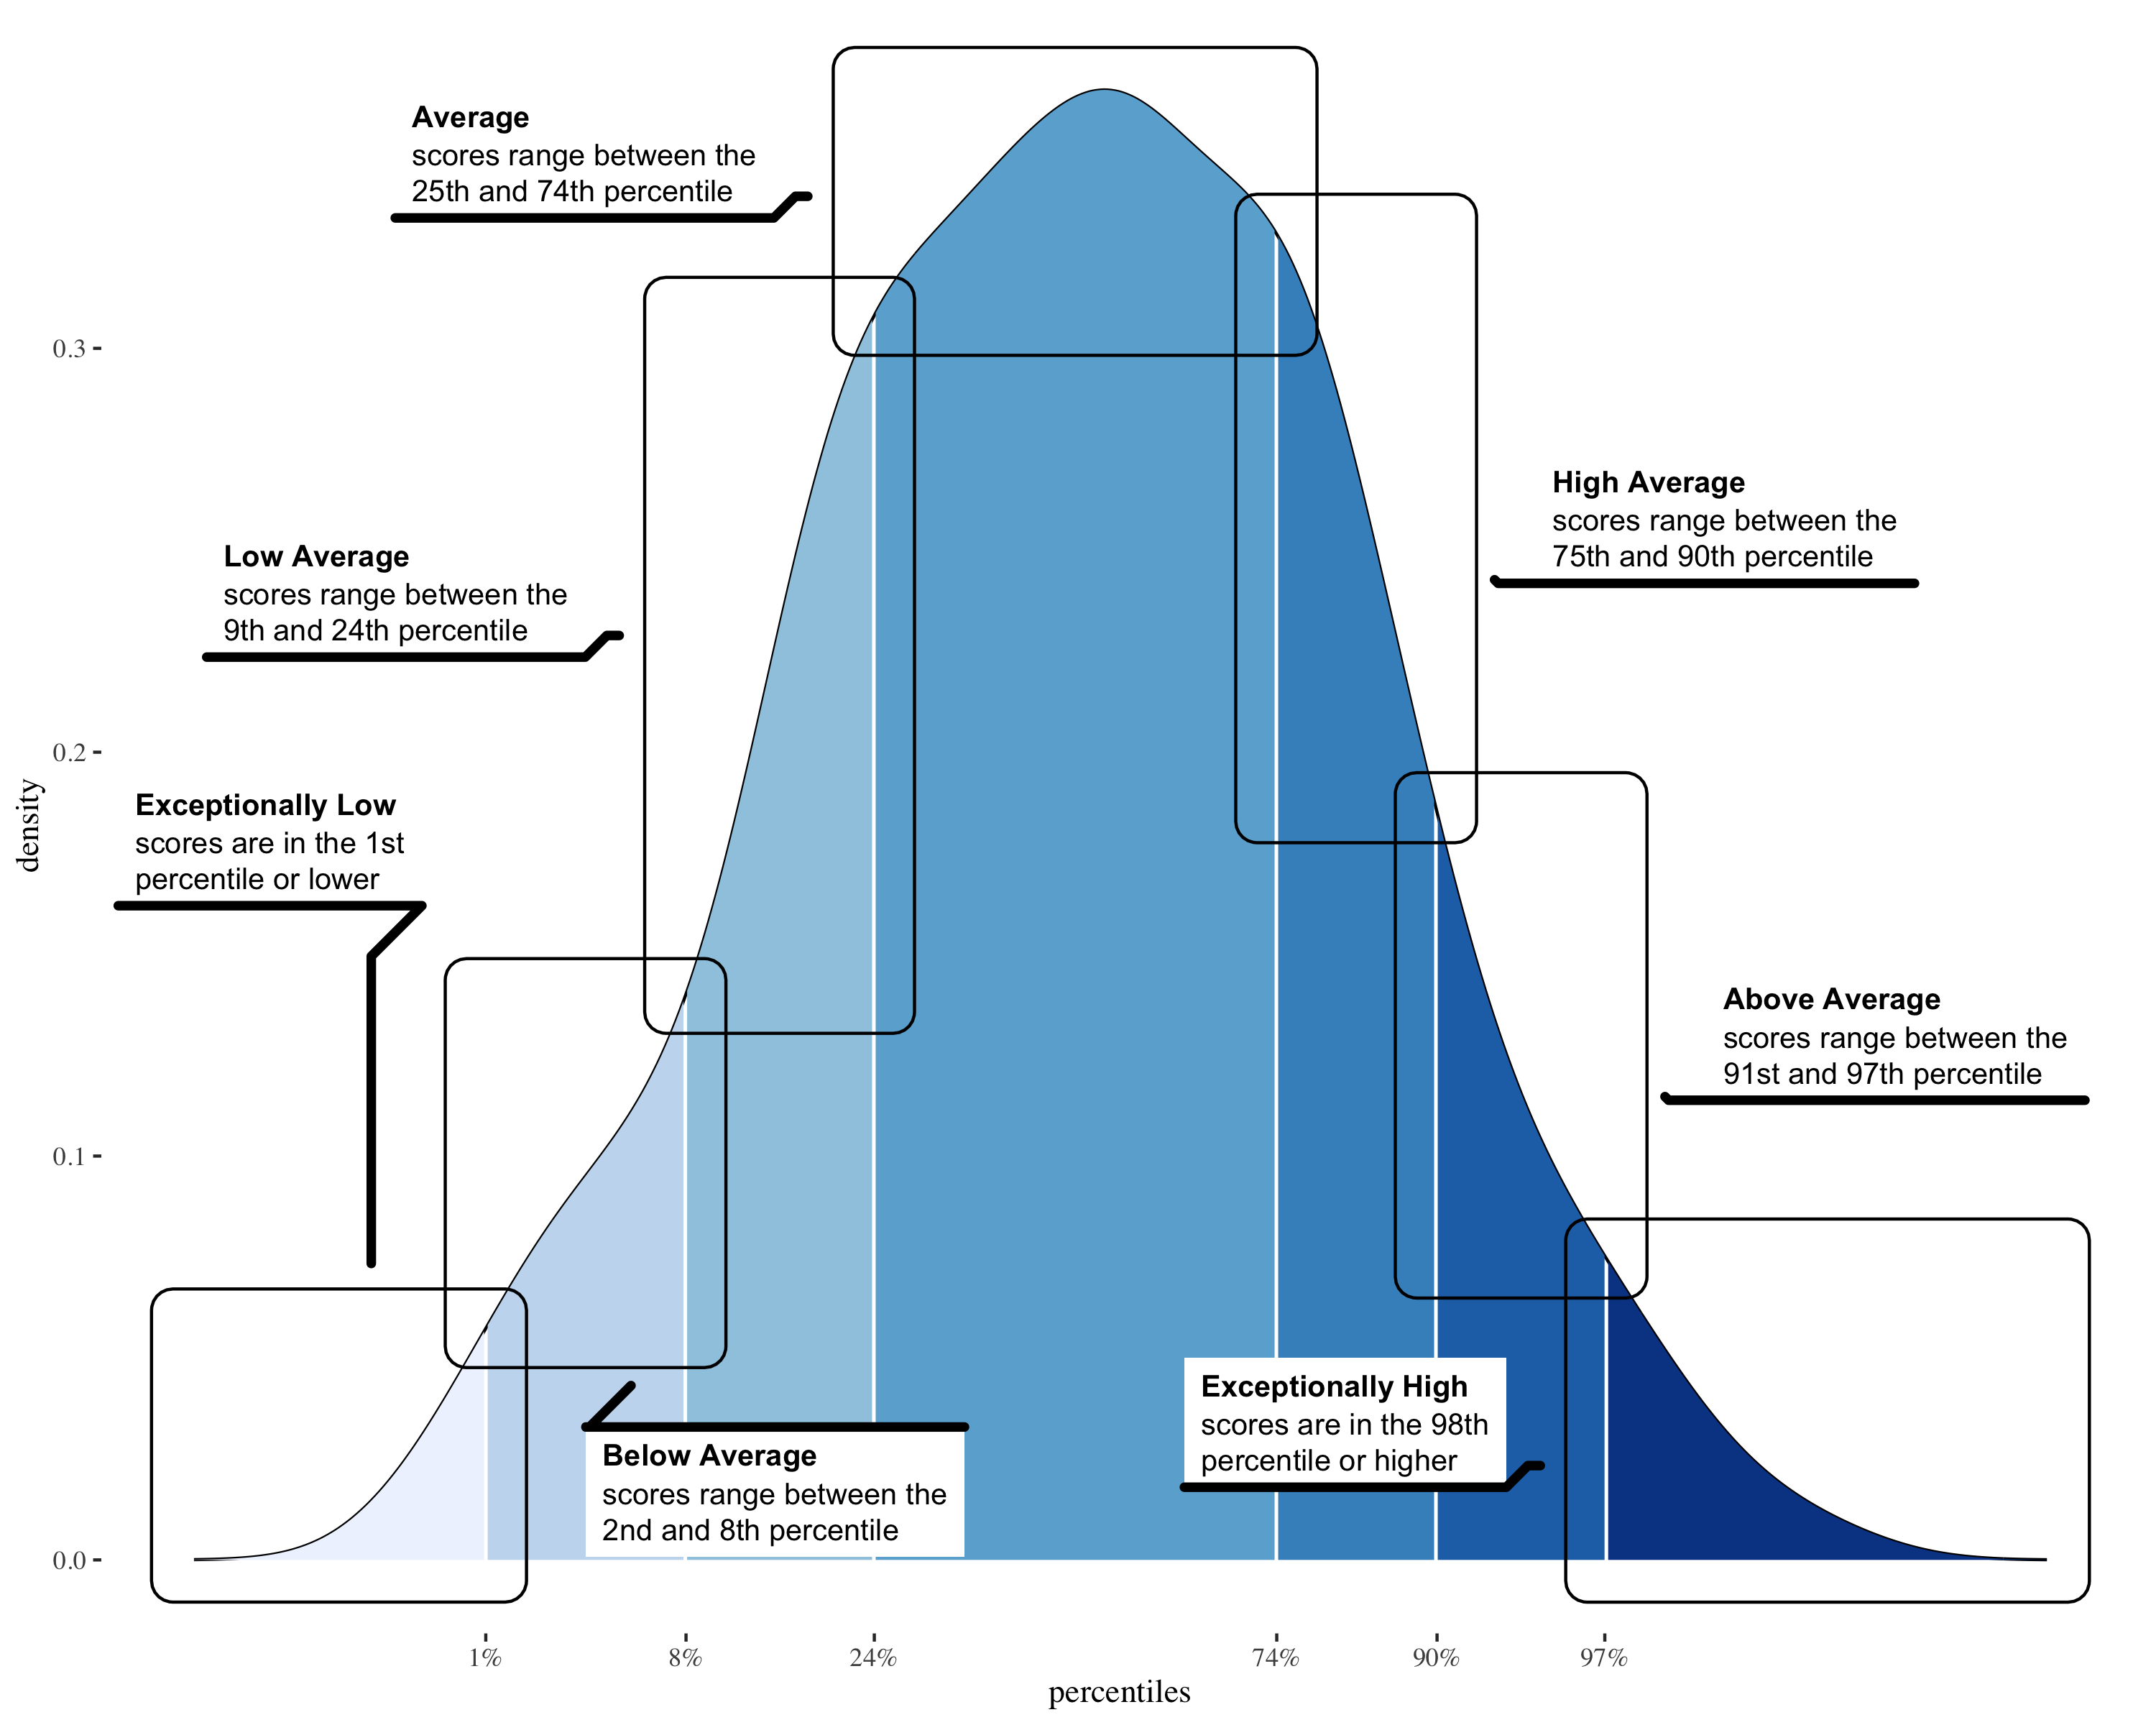
\includegraphics{plot_narrow} \caption[Statistical classification of neuropsychological test
scores in the general population \autocite{guilmetteAmericanAcademyClinical2020}.]{Statistical classification of neuropsychological test
scores in the general population \autocite{guilmetteAmericanAcademyClinical2020}.}\label{fig:gauss-plot-narrow}
\end{figure}





\begin{figure}[!ht]
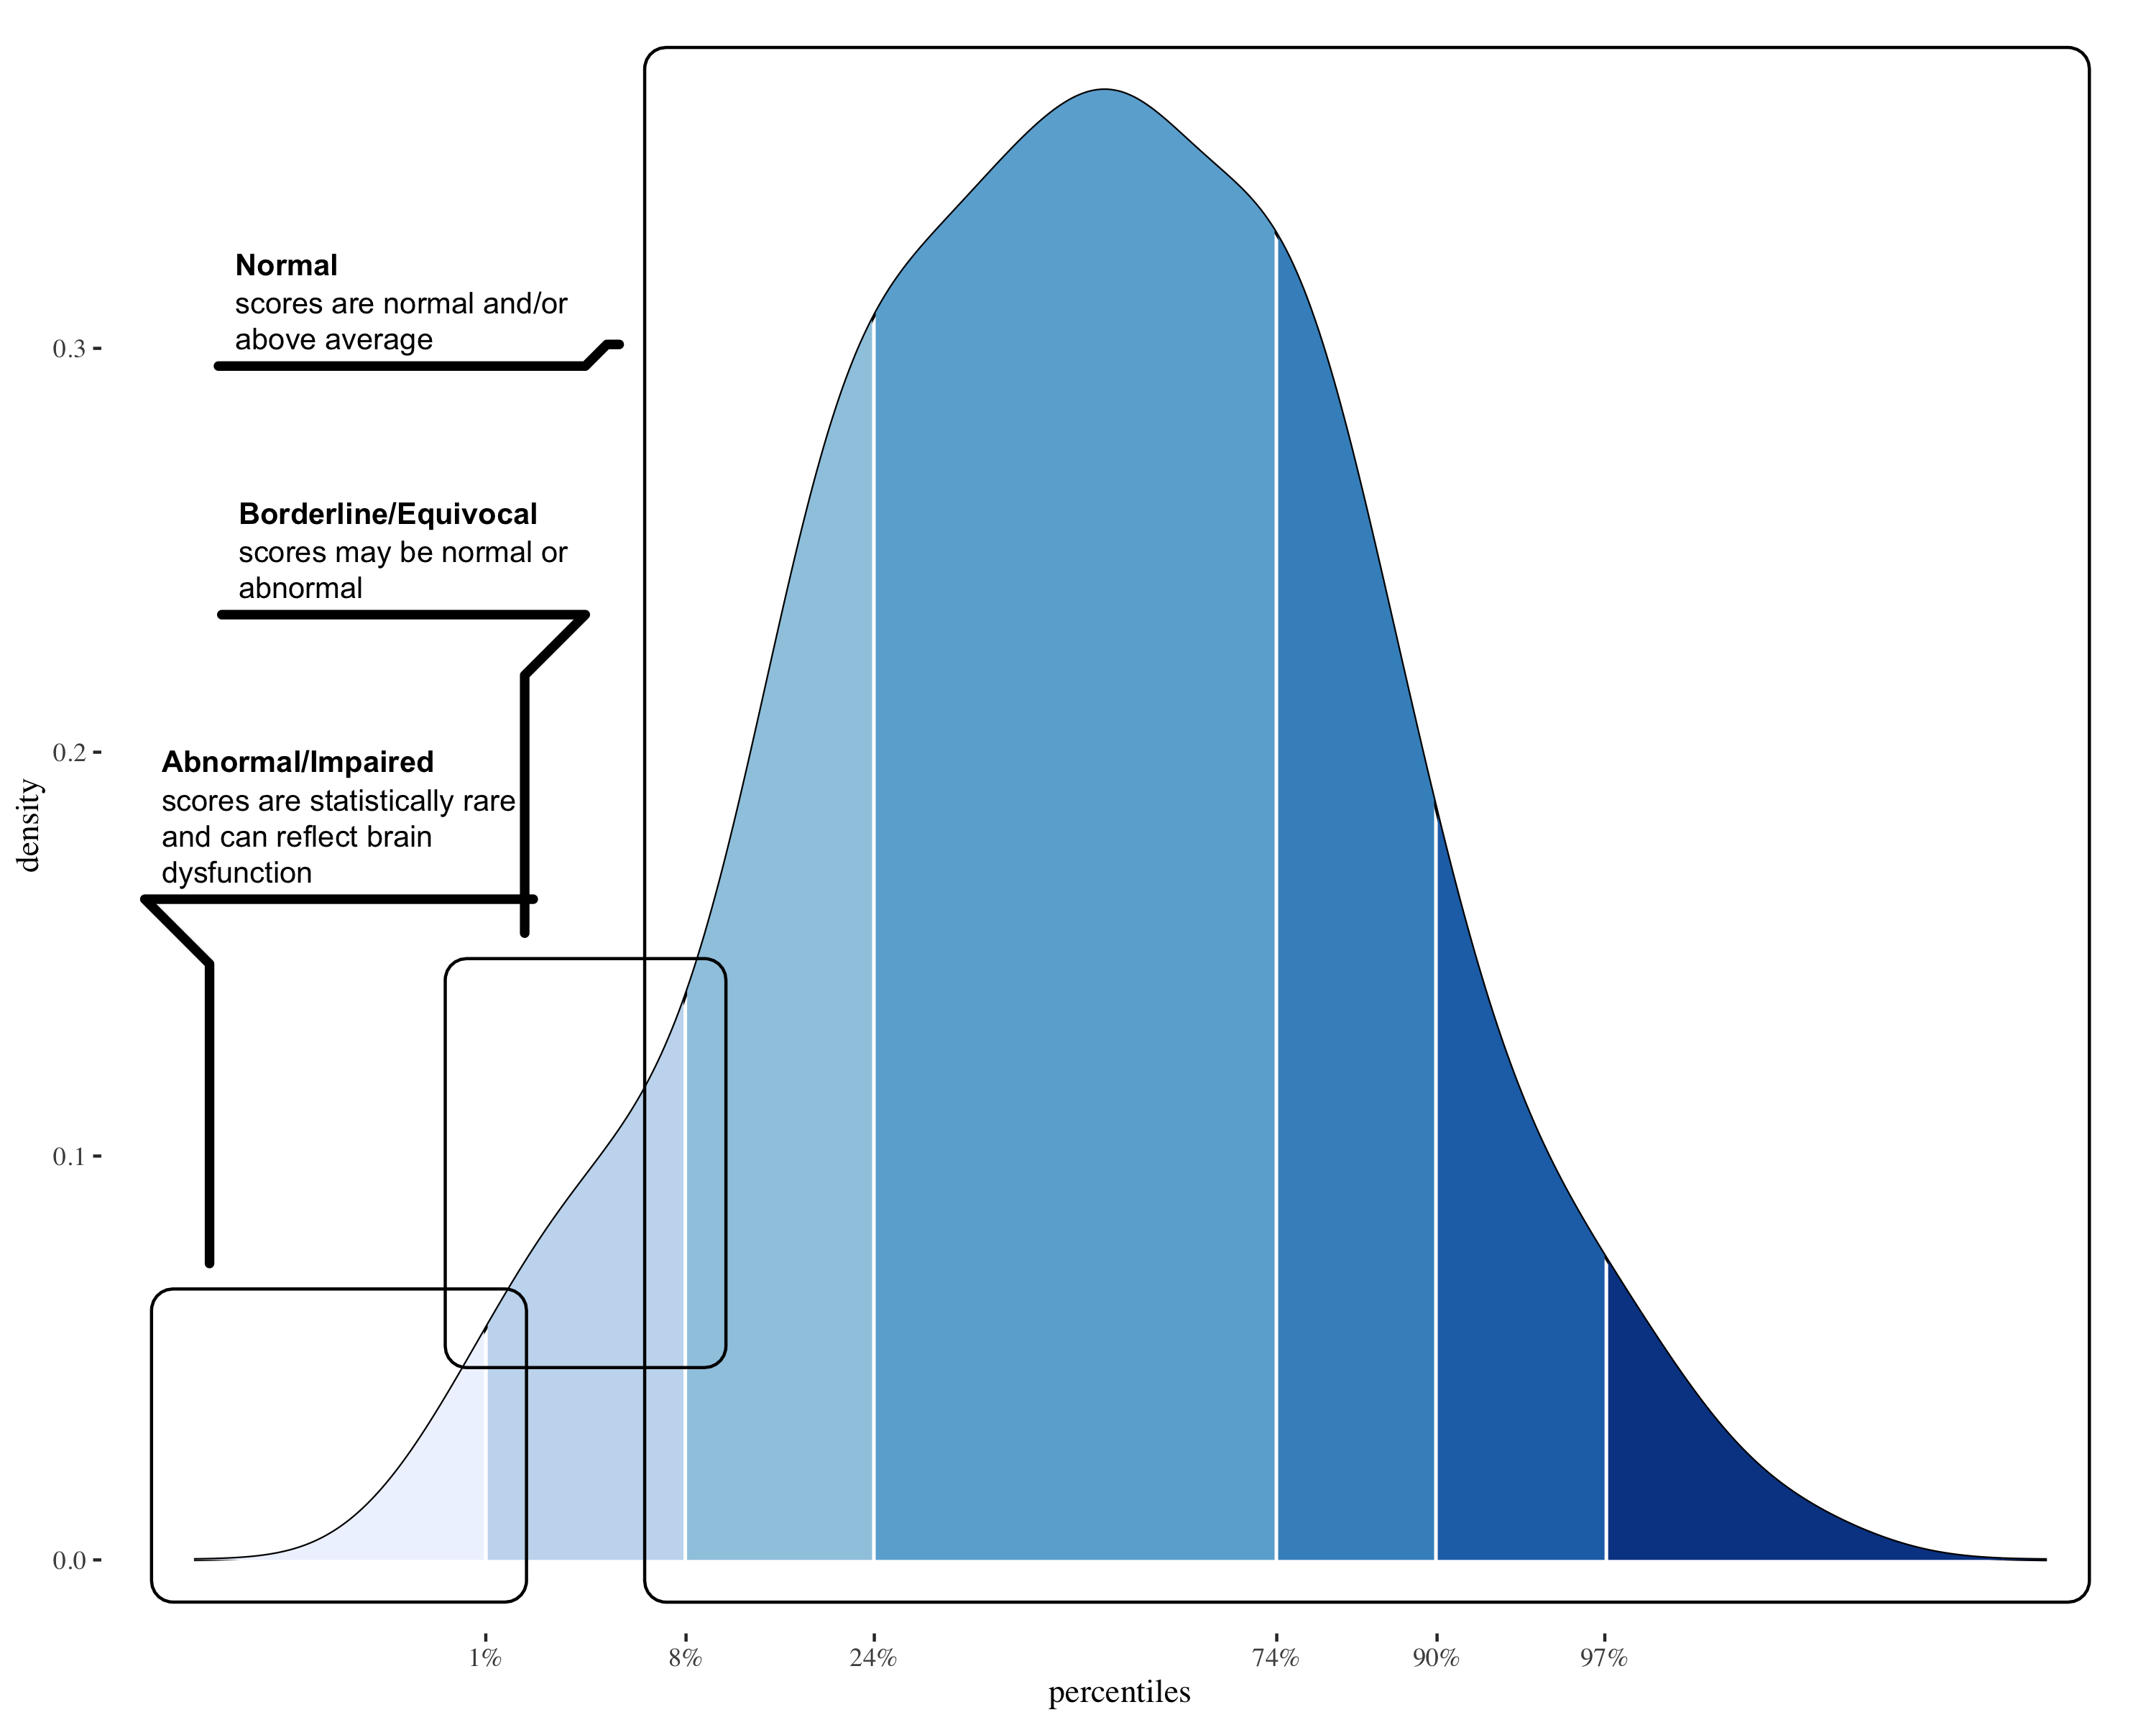
\includegraphics{plot_broad} \caption[General clinical interpretation of performance for
individual test scores and broader neuropsychological domains
\autocite{schoenbergReportingStandardsNeuropsychological2017}.]{General clinical interpretation of performance for
individual test scores and broader neuropsychological domains
\autocite{schoenbergReportingStandardsNeuropsychological2017}.}\label{fig:gauss-plot-broad}
\end{figure}

\begin{verbatim}
## Error: Problem with `filter()` input `..1`.
## x object 'percentile' not found
## i Input `..1` is `!is.na(percentile)`.
\end{verbatim}

\begin{verbatim}
## Error in dplyr::filter(., test_type == "npsych_test"): object 'neuropsych' not found
\end{verbatim}

\begin{verbatim}
## Error in dplyr::group_by(., domain, .add = TRUE): object 'neurocog' not found
\end{verbatim}

\begin{verbatim}
## Error in dplyr::group_by(., subdomain, .add = TRUE): object 'neurocog' not found
\end{verbatim}

\begin{verbatim}
## Error in dplyr::group_by(., narrow, .add = TRUE): object 'neurocog' not found
\end{verbatim}

\begin{verbatim}
## Error in dplyr::group_by(., verbal, .add = TRUE): object 'neurocog' not found
\end{verbatim}

\begin{verbatim}
## Error in dplyr::group_by(., pass, .add = TRUE): object 'neurocog' not found
\end{verbatim}

\begin{verbatim}
## Error in dplyr::group_by(., timed, .add = TRUE): object 'neurocog' not found
\end{verbatim}

\begin{verbatim}
## Error in dplyr::filter(., test_type != "npsych_test"): object 'neuropsych' not found
\end{verbatim}

\begin{verbatim}
## Error in dplyr::group_by(., domain, .add = TRUE): object 'neurobehav' not found
\end{verbatim}

\begin{verbatim}
## Error in dplyr::group_by(., subdomain, .add = TRUE): object 'neurobehav' not found
\end{verbatim}

\begin{verbatim}
## Error in dplyr::group_by(., narrow, .add = TRUE): object 'neurobehav' not found
\end{verbatim}

\begin{verbatim}
## Error in dplyr::group_by(., verbal, .add = TRUE): object 'neurobehav' not found
\end{verbatim}

\begin{verbatim}
## Error in dplyr::group_by(., pass, .add = TRUE): object 'neurobehav' not found
\end{verbatim}

\begin{verbatim}
## Error in is.data.frame(x): object 'neuropsych' not found
\end{verbatim}

\begin{verbatim}
## Error in is.data.frame(x): object 'neurocog' not found
\end{verbatim}

\begin{verbatim}
## Error in is.data.frame(x): object 'neurobehav' not found
\end{verbatim}

\begin{verbatim}
## Error: 'neuropsych.csv' does not exist in current working directory ('/Users/joey/npsych.data').
\end{verbatim}

\begin{verbatim}
## Error: 'neurocog.csv' does not exist in current working directory ('/Users/joey/npsych.data').
\end{verbatim}

\begin{verbatim}
## Error: 'neurobehav.csv' does not exist in current working directory ('/Users/joey/npsych.data').
\end{verbatim}

\newpage

\hypertarget{intelligence}{%
\subsubsection{Intelligence}\label{intelligence}}

Overall intellectual scores were \emph{high-average}. Index scores were \emph{average} to
\emph{high-average}.

\begin{verbatim}
## Error in dplyr::filter(., domain == pheno): object 'neurocog' not found
\end{verbatim}

\begin{verbatim}
## Error in knitr::kable(x = x, format = format, digits = digits, row.names = row.names, : object 'iq' not found
\end{verbatim}

\begin{verbatim}
## Error in fortify(data): object 'g' not found
\end{verbatim}

\newpage

\hypertarget{academic-skills}{%
\subsubsection{Academic Skills}\label{academic-skills}}

Biggie's academic skills were well above age- and grade-expected
levels. Written expression was \emph{exceptionally high}. Reading scores were
\emph{high-average} to \emph{above average}, with strong word reading skills.
Biggie's composite math score was \emph{high-average}, with particularly
strong math problem solving/quantitative reasoning performance.

\begin{verbatim}
## Error in dplyr::filter(., domain == pheno): object 'neurocog' not found
\end{verbatim}

\begin{verbatim}
## Error in knitr::kable(x = x, format = format, digits = digits, row.names = row.names, : object 'academics' not found
\end{verbatim}

\begin{verbatim}
## Error in dplyr::filter(., domain == "Academic Skills"): object 'neurocog' not found
\end{verbatim}

\begin{verbatim}
## Error in fortify(data): object 'acad' not found
\end{verbatim}

\newpage

\hypertarget{verballanguage}{%
\subsubsection{Verbal/Language}\label{verballanguage}}

All scores in this area were \emph{average} to \emph{above average}. An exception was
his phonemic word fluency score, which was \emph{low-average} and a
relative weakness.

\begin{verbatim}
## Error in dplyr::filter(., domain == pheno): object 'neurocog' not found
\end{verbatim}




\begin{verbatim}
## Error in knitr::kable(x = x, format = format, digits = digits, row.names = row.names, : object 'verbal' not found
\end{verbatim}

\begin{verbatim}
## Error in dplyr::filter(., domain == "Verbal/Language"): object 'neurocog' not found
\end{verbatim}

\begin{verbatim}
## Error in fortify(data): object 'vrb' not found
\end{verbatim}

\newpage

\hypertarget{visual-perceptionconstruction}{%
\subsubsection{Visual Perception/Construction}\label{visual-perceptionconstruction}}

All scores in this area were \emph{average} to \emph{above average}.

\begin{verbatim}
## Error in dplyr::filter(., domain == pheno): object 'neurocog' not found
\end{verbatim}




\begin{verbatim}
## Error in knitr::kable(x = x, format = format, digits = digits, row.names = row.names, : object 'spatial' not found
\end{verbatim}

\begin{verbatim}
## Error in dplyr::filter(., domain == "Visual Perception/Construction"): object 'neurocog' not found
\end{verbatim}

\begin{verbatim}
## Error in fortify(data): object 'spt' not found
\end{verbatim}

\newpage

\hypertarget{attentionexecutive}{%
\subsubsection{Attention/Executive}\label{attentionexecutive}}

Complex working memory and concept formation/inductive reasoning were areas of
notable strength for Biggie. Cognitive control and planning/problem
solving were about average. Verbal and spatial processing speed were variable,
but in general processing speed was one of Biggie's weakest areas on
exam. Cognitive flexibility and rapid set-shifting were areas of relative
weakness as well. Scores on timed tests varied, but tended to be weaker than on
untimed tests.

Parent reports fell in the moderately elevated range on areas of behavioral
activation (organizing, prioritizing, and activating to work), focus (focusing,
sustaining, and shifting attention to tasks), emotion regulation (managing
frustration and modulating emotions), memory (utilizing working memory and
accessing information from long-term recall), and overall executive and
attentional functioning.

\begin{verbatim}
## Error in dplyr::filter(., domain == pheno): object 'neurocog' not found
\end{verbatim}

\begin{verbatim}
## Error in knitr::kable(x = x, format = format, digits = digits, row.names = row.names, : object 'executive' not found
\end{verbatim}

\begin{verbatim}
## Error in dplyr::filter(., domain == "Attention/Executive"): object 'neurocog' not found
\end{verbatim}

\begin{verbatim}
## Error in fortify(data): object 'exe' not found
\end{verbatim}

\newpage

\hypertarget{memory}{%
\subsubsection{Memory}\label{memory}}

\begin{verbatim}
## Error in dplyr::filter(., domain == pheno): object 'neurocog' not found
\end{verbatim}




\begin{verbatim}
## Error in knitr::kable(x = x, format = format, digits = digits, row.names = row.names, : object 'memory' not found
\end{verbatim}

\begin{verbatim}
## Error in dplyr::filter(., domain == "Memory"): object 'neurocog' not found
\end{verbatim}

\begin{verbatim}
## Error in fortify(data): object 'mem' not found
\end{verbatim}

\newpage

\hypertarget{motor}{%
\subsubsection{Motor}\label{motor}}

\begin{verbatim}
## Error in dplyr::filter(., domain == pheno): object 'neurocog' not found
\end{verbatim}




\begin{verbatim}
## Error in knitr::kable(x = x, format = format, digits = digits, row.names = row.names, : object 'motor' not found
\end{verbatim}

\begin{verbatim}
## Error in dplyr::filter(., domain == "Motor"): object 'neurocog' not found
\end{verbatim}

\begin{verbatim}
## Error in fortify(data): object 'mtr' not found
\end{verbatim}

\newpage

\hypertarget{emotionalbehavioraladaptive}{%
\subsubsection{Emotional/Behavioral/Adaptive}\label{emotionalbehavioraladaptive}}

\newpage

\hypertarget{summaryimpression}{%
\section{SUMMARY/IMPRESSION}\label{summaryimpression}}









\begin{verbatim}
## Error in dplyr::filter(., test_type == "npsych_test"): object 'neurocog' not found
\end{verbatim}

\begin{verbatim}
## Error in fortify(data): object 'domain' not found
\end{verbatim}

\hypertarget{overall-evaluation-interpretation}{%
\subsection{Overall Evaluation Interpretation}\label{overall-evaluation-interpretation}}

\hypertarget{diagnostic-impression}{%
\subsection{Diagnostic Impression}\label{diagnostic-impression}}

\hypertarget{recommendations}{%
\section{RECOMMENDATIONS}\label{recommendations}}

\hypertarget{recommendations-for-medicalhealth-care}{%
\subsection{Recommendations for Medical/Health Care}\label{recommendations-for-medicalhealth-care}}

\hypertarget{recommendations-for-school}{%
\subsection{Recommendations for School}\label{recommendations-for-school}}

\hypertarget{recommendations-for-familyhome}{%
\subsection{Recommendations for Family/Home}\label{recommendations-for-familyhome}}

\hypertarget{follow-up-evaluation}{%
\subsection{Follow-Up Evaluation}\label{follow-up-evaluation}}

\begin{marginfigure}
\textbf{CONTACT}\\
\textbf{Phone:}\\
(323) 442-4000\\
\textbf{Mailing Address:}\\
USC Clinical Sciences Center, Department of Psychiatry and Behavioral
Sciences, 2250 Alcazar St., Suite 2200, Los Angeles, CA 90033\\
\textbf{Email:}\\
\href{mailto:trampush@usc.edu}{\nolinkurl{trampush@usc.edu}}\\
\end{marginfigure}

Sincerely,

\begin{flushleft}
\includegraphics[width=0.35\linewidth]{jwtSig} \end{flushleft}

\textbf{Joey Trampush, PhD}\\
Della Martin Assistant Professor of Psychiatry\\
Department of Psychiatry and the Behavioral Sciences\\
University of Southern California Keck School of Medicine\\
CA License PSY29212 \newpage

\hypertarget{appendix}{%
\section{APPENDIX}\label{appendix}}

\hypertarget{test-selection-procedures}{%
\subsection{Test Selection Procedures}\label{test-selection-procedures}}

Neuropsychological tests are intrinsically performance-based, and cognitive
performance assessed during this neuropsychological evaluation is summarized
above. Where appropriate, qualitative observations are included. Cultural
considerations were made when selecting measures, interpreting results, and
making diagnostic impressions and recommendations. Results from formal tests are
reported in comparison to other individuals the same age, sex, and educational
level as range of functioning (e.g., Below Average, Average, Above Average).
Test score labels are intended solely to be descriptive, identifying positions
of scores relative to a normal curve distribution, and should be interpreted
within the context of the patient's individual presentation and history.
Although standardized scores provide the clinician with an important and
necessary understanding of the patient's test performance compared with a
normative group, they do not on their own lead to accurate diagnosis or
treatment recommendations.

\hypertarget{conversion-of-test-scores}{%
\subsection{Conversion of Test Scores}\label{conversion-of-test-scores}}



\begin{longtable}[]{@{}lccccc@{}}
\toprule
\textbf{Score range} & \textbf{Standard score} & \textbf{\emph{T}} \textbf{score} & \textbf{Scaled score} & \textbf{\emph{z}-score} & \textbf{Percentile (‰)} \\
\midrule
\endhead
Exceptionally High & 130 + & 70 + & 16 + & 2 + & 98 + \\
Above Average & 120 -- 129 & 63 -- 69 & 14 -- 15 & 1.3 -- 1.9 & 91 -- 97 \\
High-Average & 110 -- 119 & 57 -- 62 & 12 -- 13 & 0.7 -- 1.2 & 75 -- 90 \\
Average & 90 -- 109 & 44 -- 56 & 9 -- 11 & -0.7 -- 0.6 & 25 -- 74 \\
Low-Average & 80 -- 89 & 37 -- 43 & 7 -- 8 & -1.3 -- -0.6 & 9 -- 24 \\
Below Average & 70 -- 79 & 30 -- 36 & 4 -- 6 & -2 -- -1.4 & 2 -- 8 \\
Exceptionally Low & \textless{} 70 & \textless{} 30 & \textless{} 4 & \textless{} -2 & \textless{} 2 \\
\bottomrule
\end{longtable}

\begin{fullwidth}
  \begin{multicols}{2}[\printbibheading]
    \renewcommand{\bibfont}{\small}
    \printbibliography[heading=none]
  \end{multicols}
\end{fullwidth}

\end{document}
